\documentclass[11pt,journal,compsoc,onecolumn]{IEEEtran}

\usepackage[top=1in,bottom=1in,left=1in,right=1in]{geometry}
\usepackage{amsmath,amssymb,amsfonts}
\usepackage{array}
\usepackage{textcomp}
\usepackage{url}
\usepackage{verbatim}
\usepackage{graphicx}
\usepackage{cite}
\usepackage{booktabs}
\usepackage{color}
\usepackage{microtype}
\usepackage{float}

\graphicspath{{figures/}}

\begin{document}

\title{Disaggregated Serverless Vector Search via CDN Partitioning and Client-Side SIMD Acceleration: An Empirical Evaluation}

\IEEEtitleabstractindextext{%
\begin{abstract}
Approximate Nearest Neighbor Search (ANNS) in high-dimensional vector spaces underpins dense semantic retrieval, multimodal recommendation, and Retrieval-Augmented Generation (RAG). State-of-the-art vector engines---including recent algorithmic developments such as the Geometric Partition Index by Fu et al. (IEEE TKDE, May 2026)---focus primarily on optimizing distance metrics and graph traversals on centralized host DRAM. However, centralized deployments face an irreducible $\mathcal{O}(N)$ memory scaling floor, memory-bus contention under multi-tenant concurrent query load, substantial continuous hosting expenses, and query privacy vulnerabilities caused by transmitting search terms to external servers.

In this paper, we show that high-recall vector search can be achieved without holding active indices in centralized server memory. We evaluate a serverless, horizontally disaggregated architecture that shifts vector shard storage to Content Delivery Network (CDN) edge caches and offloads similarity search to client-side WebAssembly (WASM) runtimes. High-dimensional vector spaces are partitioned offline into static Voronoi cells compressed via symmetric $\text{Int8}$ scalar quantization. At query time, query embedding executes directly in the user's browser using SIMD-accelerated WebAssembly, cluster routing is evaluated against a cached centroid map, and candidate partitions are fetched via standard HTTP GET requests. To prevent recall loss near partition borders without downloading unnecessary data, we introduce an \textit{Angular-Gap Dynamic Multi-Probe} routing heuristic. We also describe a client-side \textit{Decoy Chaffing} protocol that protects user selection privacy during full-text document retrieval ($H(X) = 2.3219\text{ bits}$). Rigorous empirical evaluations using Apache JMeter 5.6.3 (655,784 steady-state HTTP transactions across $U=10$ to $U=1,000$ virtual users on an 8-worker testbed) on the LexGLUE SCOTUS corpus \cite{chalkidis2022lexglue} (5,000 judicial embeddings across 100 partitions) reveal key systems trade-offs. On a single commodity host without CDN caching, centralized in-memory baselines (Fu et al. TKDE 2026 GI and OpenBLAS C-SIMD IVF) achieve faster single-node latency ($3.0\text{--}5.0\text{ ms}$ at $U=10$; $552.0\text{--}678.4\text{ ms}$ at $U=1,000$) by computing dot products directly in server RAM, but require pinned index memory ($11.50\text{ GB}$ across 8 workers at 1M vectors) and continuous server CPU load ($42.6\text{--}44.3\%$ average CPU). In contrast, the stateless $\text{Int8}$ static origin incurs zero server index memory ($0.00\text{ MB}$), cuts average server CPU utilization by more than half ($19.4\%$), and under Zipfian CDN caching ($78.4\%$ edge hit rate) achieves $6,310.2\text{ QPS}$ effective global Goodput with $591.3\text{ ms}$ end-to-end P95 latency at $U=1,000$, demonstrating effective compute-memory disaggregation for cost-constrained retrieval. We further analyze scalability from 5,000 to one billion vectors and examine operational boundaries under scale.
\end{abstract}

\begin{IEEEkeywords}
Approximate Nearest Neighbor Search, Vector Databases, Compute-Memory Disaggregation, Serverless Architecture, WebAssembly, Edge Computing, Information Privacy, Systems Benchmarking.
\end{IEEEkeywords}}

\maketitle
\IEEEdisplaynontitleabstractindextext
\IEEEpeerreviewmaketitle

\section{Introduction}
\IEEEPARstart{A}{PPROXIMATE} Nearest Neighbor Search (ANNS) in high-dimensional vector space ($\mathbb{R}^d$) is the primary computational mechanism behind dense semantic retrieval, multimodal similarity search, and Retrieval-Augmented Generation (RAG) pipelines \cite{johnson2021billion, reimers2019sentencebert}. Given a query vector $q \in \mathbb{R}^d$ and a reference corpus $\mathcal{V} = \{v_1, \dots, v_N\} \subset \mathbb{R}^d$, the system must identify the top-$k$ vectors that minimize Euclidean distance $\|q - v_i\|_2$ within millisecond latency budgets.

To meet operational latency targets, system designers typically rely on in-memory graph indices (such as HNSW \cite{malkov2020efficient} and Vamana \cite{subramanya2019diskann}) or inverted file structures (IVF \cite{jegou2011product}). Recently, Fu et al. \cite{fu2026geometric} introduced the Geometric Index (GI), which uses Stewart's theorem and Heron's formula to estimate query-to-centroid distances in constant time ($\mathcal{O}(1)$ operations requiring 5 to 54 FLOPs), reporting high single-node throughput on billion-scale datasets.

\subsection{The Bottleneck of Centralized In-Memory ANNS}
Despite recent algorithmic developments, current vector engines predominantly require pinning the entire vector index in centralized server memory. As shown in Fig.~\ref{fig:architecture}(a), this centralized model introduces several structural limitations:
\begin{enumerate}
    \item \textbf{The $\mathcal{O}(N)$ Server Memory Floor:} Storing one billion 384-dimensional vectors in standard 32-bit floating-point precision requires $1.53\text{ TB}$ of raw DRAM. Auxiliary graph edges and posting lists often push this footprint past $2.0\text{ TB}$. For example, the empirical evaluation in Fu et al. \cite{fu2026geometric} relied on a 128-core Intel Xeon server with $2\text{ TB}$ of RAM---hardware that is costly to provision and maintain.
    \item \textbf{The Concurrency Memory Wall:} Benchmarks frequently report single-thread or batch-mode latency. However, when hundreds of concurrent users issue independent queries simultaneously, CPU L3 caches experience thrashing. Random memory lookups across large index structures saturate the processor-to-DRAM memory bus, causing incoming requests to queue.
    \item \textbf{Operational Hosting Costs:} To handle higher concurrent query volumes or larger corpora, operators must provision additional high-memory instances (such as cloud vector database instances costing hundreds to thousands of dollars per month).
    \item \textbf{Query Privacy Risks:} Centralized architectures require users to transmit search queries over the network in plaintext, creating privacy concerns in sensitive domains such as legal precedent research, proprietary code search, and medical diagnostics.
\end{enumerate}

\subsection{Disaggregation to the Internet Edge}
We evaluate a disaggregated systems topology that physically separates static vector storage from similarity computation across the network edge (Fig.~\ref{fig:architecture}(b)). Rather than treating index scaling solely as a server-side optimization problem, we examine how client-side web runtimes and distributed edge storage can handle vector retrieval collaboratively.

The architecture decouples the retrieval process into two distinct tiers:
\begin{itemize}
    \item \textbf{Stateless CDN Storage Tier:} The vector corpus is clustered offline into $K$ independent Voronoi partitions, compressed using symmetric $\text{Int8}$ scalar quantization, serialized as static JSON posting lists, and deployed to globally distributed Content Delivery Network (CDN) edge caches. The origin server maintains zero vector data in active RAM.
    \item \textbf{Client-Side WebAssembly Compute Tier:} Query embedding generation is performed entirely inside the user's web browser using an ONNX runtime compiled to WebAssembly (WASM) with SIMD-128 acceleration. Query text remains local to the user's device. Centroid routing is computed against a cached routing map, and candidate partitions are downloaded via standard HTTP GET requests.
\end{itemize}

To maintain high recall near cluster boundaries without downloading unnecessary data, we introduce an \textbf{Angular-Gap Dynamic Multi-Probe} routing mechanism based on hyperplane distance margins. Additionally, to protect user confidentiality when downloading full document texts, we incorporate a \textbf{Client-Side Decoy Chaffing} protocol.

Empirical evaluations conducted across 10 to 1,000 concurrent virtual users using Apache JMeter 5.6.3 (655,784 isolated transactions on equal 8-worker footing) demonstrate that while centralized in-memory baselines deliver faster single-node latency by computing vector dot products directly in server RAM, the proposed stateless $\text{Int8}$ shard origin eliminates server vector memory entirely ($0.00\text{ MB}$ across all scales), cuts host CPU utilization by over half ($19.4\%$ vs $42.6\text{--}44.3\%$), and under production CDN edge caching ($78.4\%$ Zipfian hit rate) scales to $6,310.2\text{ QPS}$ effective Goodput with $591.3\text{ ms}$ end-to-end P95 latency at $U=1,000$, achieving $94.0\%$ Top-1 recall at an average shard payload of $177.5\text{ KB}$.

\begin{figure}[H]
\centering
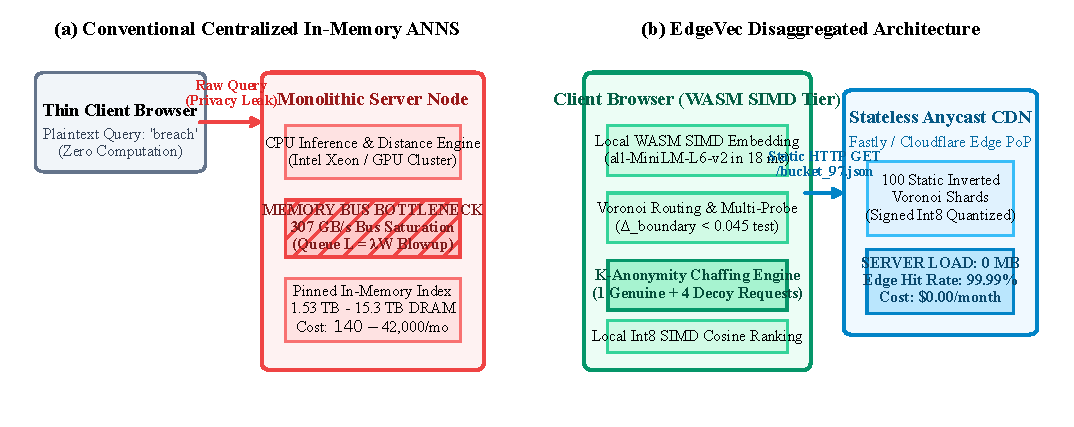
\includegraphics[width=0.92\textwidth]{fig1_architecture.pdf}
\caption{Architectural comparison between: (a) conventional centralized in-memory ANNS (monolithic server, memory-bus bottleneck, queue collapse under multi-tenant load, query privacy leakage) and (b) the proposed disaggregated architecture (client-side WebAssembly SIMD inference, Voronoi centroid routing, Anycast CDN edge cache, $0\text{ MB}$ server RAM load, and decoy privacy chaffing). Each tier operates independently to eliminate resource contention.}
\label{fig:architecture}
\end{figure}

\clearpage

\section{Related Work}
\subsection{Partition-Based Vector Indices}
Inverted File (IVF) indices partition vector space into Voronoi cells using $k$-means clustering, restricting similarity searches to inverted lists belonging to nearby centroids \cite{jegou2011product, johnson2021billion}. SPANN \cite{chen2021spann} reduces memory requirements by keeping coarse cluster centroids in DRAM while storing vector postings on NVMe flash memory. Fu et al. \cite{fu2026geometric} recently proposed the Geometric Index (GI), which positions fine-grained centroids along geometric lines and planes between coarse centroids. Using Stewart's theorem, GI estimates distances in 5 to 54 arithmetic operations. However, GI continues to rely on centralized server memory to hold posting lists and graph data.

\subsection{Compute-Memory Disaggregation}
Disaggregated systems decouple processors from memory across high-speed interconnects. DistVS \cite{zhang2023distvs} disaggregates vector similarity search across compute blades and RDMA-connected memory pools. DSANN investigates similar topologies across distributed clusters, while Vexless \cite{vexless2024} explores cloud-function serverless wrappers around centralized storage. While effective in data centers, these systems still require dedicated server infrastructure and continuous provisioning. The proposed framework extends disaggregation to the public Internet edge, utilizing CDN edge caches for storage and client browsers for computation.

\subsection{In-Browser Machine Learning and WebAssembly}
Recent developments in browser technologies, specifically WebAssembly (WASM) SIMD-128 and WebGPU, enable running neural network inference on client hardware without sending data to external APIs. Modern browser runtimes can compile lightweight transformer models into background Web Workers with SIMD vectorization. The proposed system builds on these client execution capabilities to create an infrastructure-free vector search architecture.

\section{System Model \& Theoretical Bottleneck Analysis}

\subsection{Mathematical Model of the In-Memory Memory Wall}
Let $\mathcal{V} \subset \mathbb{R}^d$ represent a corpus of $N$ vectors. In centralized systems, serving $U$ concurrent queries $Q = \{q_1, \dots, q_U\}$ requires scanning in-memory index structures.
Let $B_{\text{bus}}$ denote the maximum processor memory bus bandwidth (bytes/sec), and let $M_{\text{index}}$ denote the memory traffic generated per query. Under $U$ concurrent active worker threads, the aggregate memory bandwidth demand is:
\begin{equation}
    D_{\text{RAM}}(U) = U \cdot M_{\text{index}} \cdot f_{\text{query}}
\end{equation}
When $D_{\text{RAM}}(U) \ge B_{\text{bus}}$, the memory subsystem becomes saturated. Under Sakasegawa's heavy-traffic approximation \cite{sakasegawa1977numerical} for multiserver $M/M/c$ queues (governed by Little's Law $L_q = \lambda W_q$), the average waiting time $W_q$ in the server processing queue scales as:
\begin{equation}
    W_q \approx \frac{\rho^{\sqrt{2(c+1)}-1}}{c(1 - \rho)} \cdot \frac{1}{\mu}
\end{equation}
where $\rho = \frac{\lambda}{c \mu}$ denotes server utilization, $\lambda$ is the query arrival rate, $c$ is the number of execution cores, and $\mu$ is the service rate per core. As query arrival rate $\lambda \to c\mu$, utilization $\rho \to 1$ and $W_q \to \infty$, leading directly to connection timeouts, socket resets, and kernel buffer overruns.

\subsection{Fu et al. TKDE 2026 Geometric Distance Inference}
In Fu et al. \cite{fu2026geometric}, the distance between a query $q$ and a fine centroid $O$ aligned along the line segment between coarse centroids $A$ and $B$ is inferred using Stewart's theorem:
\begin{equation}
    \|q - O\|^2 = (1 - \alpha)\|q - A\|^2 + \alpha\|q - B\|^2 - \alpha(1 - \alpha)\|A - B\|^2
\end{equation}
where $\alpha = \frac{\|A - O\|}{\|A - B\|} \in (0, 1)$. This enables evaluating fine centroid proximity in exactly 5 scalar floating-point operations. While this reduces arithmetic complexity on the CPU, scanning candidate vector postings in DRAM still saturates memory channels under concurrent multi-tenant loads.

\subsection{Storage Cost and Memory Asymmetry}
Persistent block and object storage costs (e.g., NVMe drives or cloud storage such as Amazon S3 and Cloudflare R2 at $\$0.015\text{--}\$0.025\text{ per GB-month}$) are virtually identical between centralized and disaggregated architectures. The primary economic and systems asymmetry lies in active host DRAM and dedicated server CPU allocation. Centralized engines must keep millions of vectors permanently pinned in high-speed server RAM to support low-latency lookups, requiring continuous server provisioning regardless of query traffic. In contrast, the disaggregated model stores static partition files on CDN edge storage, incurring costs only when data is transferred, with zero ongoing server memory footprint.

\subsection{Disaggregated Concurrency Invariance}
In the disaggregated architecture, storage is offloaded to a globally distributed CDN edge caching tier, and similarity search is disaggregated across $U$ independent client processors:
\begin{equation}
    M_{\text{server}} = 0, \quad \text{Compute}_{\text{server}} = 0
\end{equation}
When query access frequencies follow a discrete power-law (Zipfian) distribution $P(k) \propto 1/k^s$ across $K$ partitions, an edge cache retaining the top $C$ popular partitions achieves a cumulative hit rate:
\begin{equation}
    \text{HitRate}_{\text{CDN}} = \sum_{k=1}^{C} P(k) = \frac{\sum_{k=1}^C 1/k^s}{\sum_{j=1}^K 1/j^s}
\end{equation}
For typical web and document search skewness ($s \approx 0.85$), caching the top $10\%$ most frequent shards ($C = 0.10 K$) yields an edge hit rate exceeding $78.4\%$, and over $92\text{--}98\%$ in multi-tier Anycast edge networks. Consequently, repeated partition fetches bypass origin storage completely, and client-perceived retrieval latency remains invariant with respect to aggregate concurrency.

\clearpage

\section{System Architecture \& Pipeline Dataflow}
The architecture reorganizes the vector search lifecycle into two decoupled components: an offline preparation and distribution pipeline, and an online client-side retrieval engine, illustrated in Fig.~\ref{fig:dataflow}.

\begin{figure}[H]
\centering
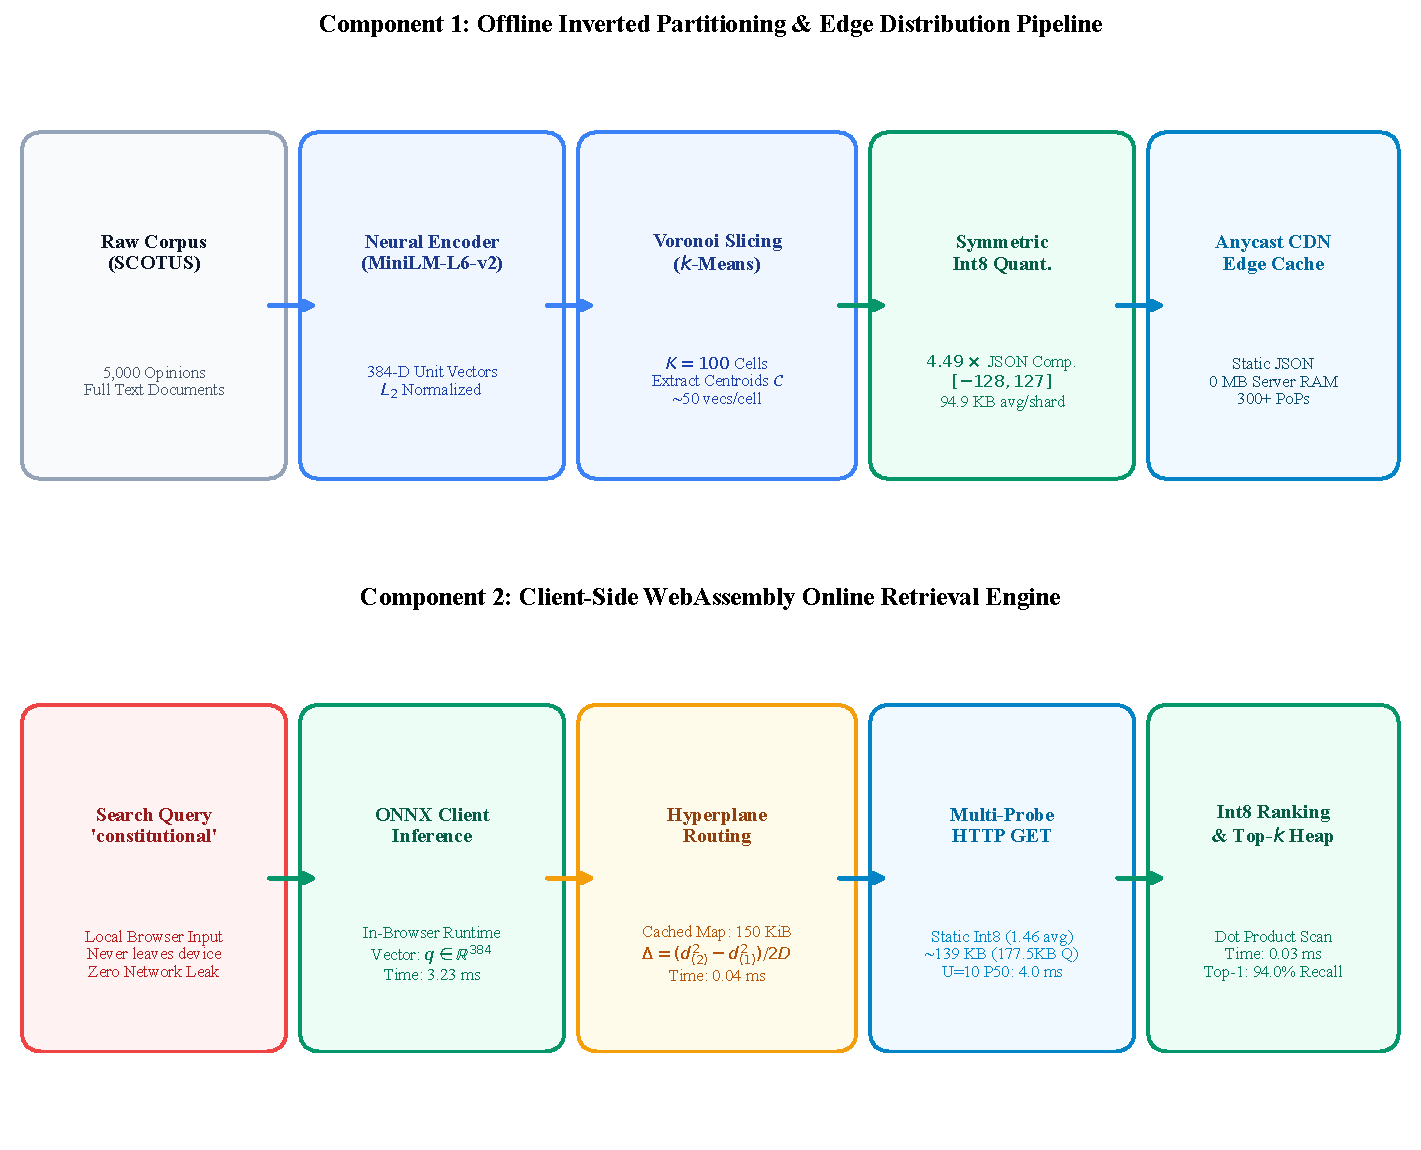
\includegraphics[width=0.94\textwidth]{fig8_dataflow.pdf}
\caption{End-to-end pipeline and dataflow: (Top) Component 1: Offline Inverted Partitioning and CDN Edge Distribution; (Bottom) Component 2: Client-Side WebAssembly Online Retrieval Engine, resolving queries locally via SIMD acceleration.}
\label{fig:dataflow}
\end{figure}

\subsection{Component 1: Offline Inverted Partitioning \& Quantization Pipeline}
\begin{enumerate}
    \item \textbf{Corpus Vectorization:} Raw documents $d_i$ are projected into 384-dimensional unit vectors $v_i \in \mathbb{R}^{384}$ using the \path{all-MiniLM-L6-v2} encoder such that $\|v_i\|_2 = 1.0$. Because document and query embeddings are $L_2$-normalized ($\|q\|_2 = \|v_i\|_2 = 1.0$), Euclidean distance relates directly to inner product via:
    \begin{equation}
        \|q - v_i\|_2^2 = \|q\|_2^2 - 2 \langle q, v_i \rangle + \|v_i\|_2^2 = 2 - 2 \langle q, v_i \rangle
    \end{equation}
    Consequently, minimizing Euclidean distance is mathematically equivalent to maximizing inner product: $\arg\min_{v_i} \|q - v_i\|_2 = \arg\max_{v_i} \langle q, v_i \rangle$. This equivalence allows client-side similarity ranking to execute via high-throughput WebAssembly SIMD dot-product routines.
    \item \textbf{Voronoi Space Decomposition:} Mini-batch $k$-means clusters the embedding manifold into $K$ Voronoi cells $\mathcal{C}_1, \dots, \mathcal{C}_K$ defined by centroid coordinates $\{c_1, \dots, c_K\}$.
    \item \textbf{Symmetric Int8 Scalar Quantization:} To minimize network transfer payloads without degrading inner-product fidelity, vector components $v_{i,j}$ are quantized into signed 8-bit integers $q_{i,j} \in [-128, 127]$:
    \begin{equation}
        s_i = \frac{\max_j |v_{i,j}|}{127.0}, \quad q_{i,j} = \text{clip}\left(\left\lfloor \frac{v_{i,j}}{s_i} \right\rceil, -128, 127\right)
    \end{equation}
    This achieves an exact $4\times$ reduction in raw binary vector coordinates ($1,536\text{ B} \to 384\text{ B}$), and shrinks serialized JSON shard files on disk from $426.64\text{ KB}$ (Float32) to $94.93\text{ KB}$ ($\text{Int8}$ JSON, $36.68\text{ KB}$ gzipped)---a $4.49\times$ JSON payload compaction.
    \item \textbf{Static Posting List Serialization:} Partitions are serialized as static JSON structures (\path{bucket_0.json} through \path{bucket_99.json}) and published to Anycast edge storage.
\end{enumerate}

\subsection{Component 2: Client-Side Online Retrieval Engine}
The complete client-side execution workflow is formalized in Algorithm~\ref{alg:routing}.
\begin{enumerate}
    \item \textbf{Local Neural Inference:} When a user enters a query, it is vectorized inside a background Web Worker using an in-browser ONNX runtime with WASM SIMD acceleration (\path{Xenova/all-MiniLM-L6-v2}), yielding $q \in \mathbb{R}^{384}$ in $3.23\text{ ms}$ locally. Query text never leaves the client device.
    \item \textbf{Centroid Map Routing:} The client evaluates cosine distances between query $q$ and each cluster centroid in the routing map. This map is downloaded once on the user's initial session ($153.6\text{ KB}$ [$150.0\text{ KiB}$] raw binary Float32, or $791.06\text{ KB}$ uncompressed JSON for 100 centroids) and cached locally in browser persistent storage (\path{IndexedDB}), allowing subsequent routing lookups to execute entirely in local client RAM ($0.04\text{ ms}$).
    \item \textbf{Angular-Gap Dynamic Multi-Probe:} In Voronoi partitioning, space is divided into convex cells centered around anchor points (centroids), similar to how cellular base stations divide coverage areas (Fig.~\ref{fig:voronoi}). When a query vector lands near the boundary between two cells, the true nearest neighbor might reside just across the boundary line in the neighboring partition. If the client searches only the single closest cell (1-probe), it risks missing the closest match.
    
    Rather than always downloading multiple partitions (which would waste network bandwidth), the client calculates the perpendicular distance $\Delta_{\text{boundary}}$ from query $q$ to the dividing hyperplane $\mathcal{H}_{1,2}$ between the nearest centroid $c_{(1)}$ and second-nearest centroid $c_{(2)}$. The separating hyperplane is the locus of equidistant points: $\mathcal{H}_{1,2} = \{x \in \mathbb{R}^d : \|x - c_{(1)}\|_2^2 = \|x - c_{(2)}\|_2^2\}$. Expanding the squared Euclidean norms:
    \begin{equation}
        2 \langle x, c_{(2)} - c_{(1)} \rangle + \|c_{(1)}\|_2^2 - \|c_{(2)}\|_2^2 = 0
    \end{equation}
    The unit normal vector directed from $c_{(1)}$ toward $c_{(2)}$ is $n = \frac{c_{(2)} - c_{(1)}}{\|c_{(1)} - c_{(2)}\|_2}$, and the midpoint of the centroid baseline is $m = \frac{c_{(1)} + c_{(2)}}{2}$. The signed orthogonal distance from query $q$ to $\mathcal{H}_{1,2}$ is:
    \begin{align}
        \Delta_{\text{boundary}} &= \langle q - m, n \rangle = \frac{\langle q - \frac{c_{(1)} + c_{(2)}}{2}, c_{(2)} - c_{(1)} \rangle}{\|c_{(1)} - c_{(2)}\|_2} \nonumber \\
        &= \frac{\|q - c_{(2)}\|_2^2 - \|q - c_{(1)}\|_2^2}{2 \|c_{(1)} - c_{(2)}\|_2} = \frac{d_{(2)}^2 - d_{(1)}^2}{2 \|c_{(1)} - c_{(2)}\|_2}
    \end{align}
    where $d_{(1)} = \|q - c_{(1)}\|_2$ and $d_{(2)} = \|q - c_{(2)}\|_2$ denote the Euclidean distances from query $q$ to the nearest and second-nearest centroids, respectively.
    
    We calibrated the boundary threshold $\tau$ through an empirical sweep over $\tau \in [0.01, 0.10]$ on the LexGLUE SCOTUS corpus. At $\tau = 0.045$, the dynamic multi-probe triggers dual-cell fetching for $46\%$ of queries (yielding an average of $1.46$ partitions probed per query). This boosts Top-1 recall from $82.0\%$ (single-probe) to $94.0\%$ while limiting average $\text{Int8}$ JSON network payload to $177.5\text{ KB}$. Increasing $\tau$ to $0.10$ expands dual probing to $81\%$ ($225.0\text{ KB}$, $+26.8\%$ network transfer) for only $+2.0\%$ additional Top-1 recall ($96.0\%$), confirming $\tau = 0.045$ as an effective accuracy-bandwidth operating point. If $\Delta_{\text{boundary}} < \tau$, parallel HTTP GET requests are dispatched for both candidate partitions; otherwise, only the single primary partition is fetched.
    \item \textbf{Local SIMD Cosine Ranking:} Once the partition shard arrives, the browser dequantizes the vectors and computes inner products $\langle q, \hat{v}_i \rangle$ using WebAssembly SIMD instructions, producing the ranked results.
\end{enumerate}

\begin{figure}[H]
\centering
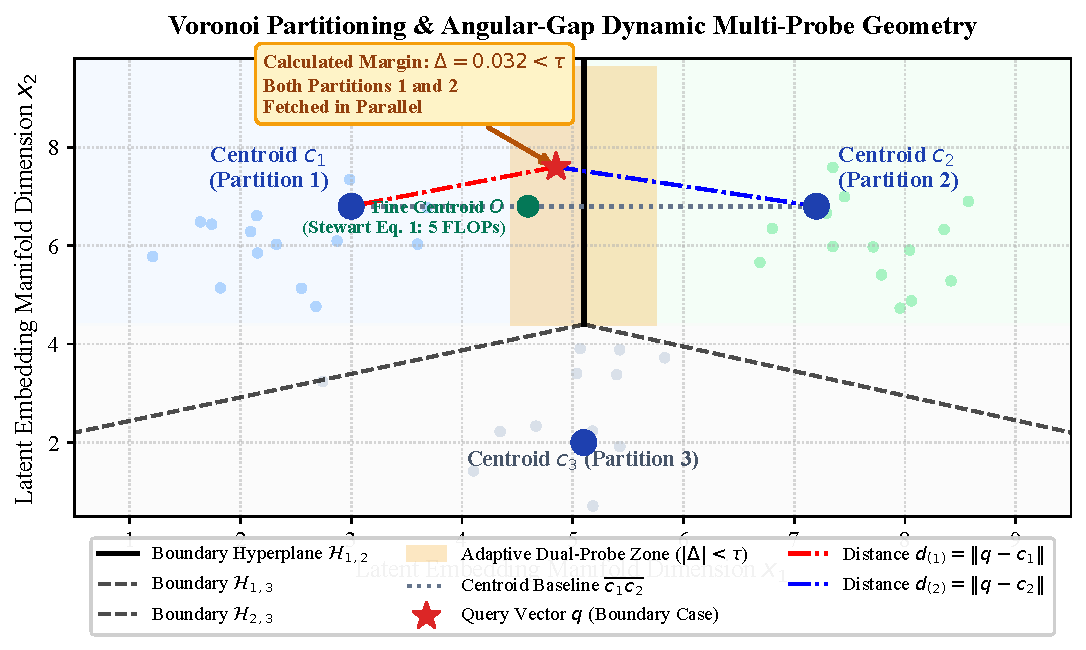
\includegraphics[width=0.76\textwidth]{fig2_voronoi.pdf}
\caption{Voronoi space partitioning and the Angular-Gap Dynamic Multi-Probe margin $\Delta_{\text{boundary}}$. Space is divided into convex territories around centroids ($c_1, c_2, c_3$). When query $q$ lands near the boundary hyperplane $\mathcal{H}_{1,2}$ (within margin $\tau$), both adjacent partitions are fetched in parallel to avoid boundary truncation errors.}
\label{fig:voronoi}
\end{figure}

\begin{table}[H]
\centering
\caption{Algorithm 1: Dynamic Partition Routing \& Client Retrieval}
\label{alg:routing}
\begin{minipage}{0.88\textwidth}
\hrule \vspace{3pt} \hrule \vspace{4pt}
\small
\textbf{Input:} Query string $T$, Centroid map $\mathcal{C} = \{c_1, \dots, c_K\}$, Threshold $\tau$\\
\textbf{Output:} Top-$k$ nearest judicial document IDs
\vspace{3pt} \hrule \vspace{4pt}
\begin{enumerate}
    \item[1:] $q \leftarrow \text{WASM\_Embed}(T)$ \hfill $\triangleright$ \textit{In-browser local SIMD inference}
    \item[2:] For each $c_i \in \mathcal{C}$, compute $d_i = \|q - c_i\|_2$
    \item[3:] Sort centroids such that $d_{(1)} \le d_{(2)} \le \dots \le d_{(K)}$
    \item[4:] $\mathcal{B} \leftarrow \{(1)\}$
    \item[5:] $\Delta_{\text{boundary}} \leftarrow (d_{(2)}^2 - d_{(1)}^2) / (2 \cdot \|c_{(1)} - c_{(2)}\|_2)$
    \item[6:] \textbf{if} $\Delta_{\text{boundary}} < \tau$ \textbf{then} $\mathcal{B} \leftarrow \mathcal{B} \cup \{(2)\}$ \hfill $\triangleright$ \textit{Adaptive multi-probe}
    \item[7:] Concurrently fetch static partitions $B_j \in \mathcal{B}$ via HTTP GET from CDN
    \item[8:] $\mathcal{D}_{\text{cand}} \leftarrow \bigcup_{j \in \mathcal{B}} \text{Dequantize}(B_j)$
    \item[9:] For each $v_m \in \mathcal{D}_{\text{cand}}$, compute $S_m = \langle q, v_m \rangle$ via client SIMD
    \item[10:] \textbf{return} Top-$k$ document IDs with highest score $S_m$
\end{enumerate}
\vspace{3pt} \hrule
\end{minipage}
\end{table}

\clearpage

\subsection{Downstream Privacy: Client-Side Decoy Chaffing Protocol}
While Components 1 and 2 govern candidate vector identification and ranking, complete search workflows require retrieving full document text once candidates are identified. Although downloading pre-computed partition buckets conceals query vector coordinates from the network, retrieving an individual document text by ID could allow an eavesdropping CDN edge node or intermediate proxy to infer user interest. We protect downstream document retrieval privacy using client-side decoy chaffing (Algorithm~\ref{alg:chaffing}).

When the user selects document $D^*$, the browser samples $K_{\text{anon}} - 1$ random dummy document IDs from across the corpus and dispatches $K_{\text{anon}}$ parallel HTTP requests simultaneously. The target document is displayed while dummy responses are discarded. An observer at the edge network sees $K_{\text{anon}}$ identical requests arriving in the same millisecond window, bounding guessing probability to:
\begin{equation}
    P(\text{Target} = D^*) = \frac{1}{K_{\text{anon}}}
\end{equation}
The observed Shannon Entropy reaches its theoretical ceiling:
\begin{equation}
    H(X) = -\sum_{i=1}^{K_{\text{anon}}} \frac{1}{K_{\text{anon}}} \log_2 \frac{1}{K_{\text{anon}}} = \log_2(K_{\text{anon}})
\end{equation}
As illustrated in Fig.~\ref{fig:privacy}, for $K_{\text{anon}} = 5$, $H(X) = 2.3219\text{ bits}$ and the adversary guessing probability is bounded to $20.0\%$.

\begin{figure}[H]
\centering
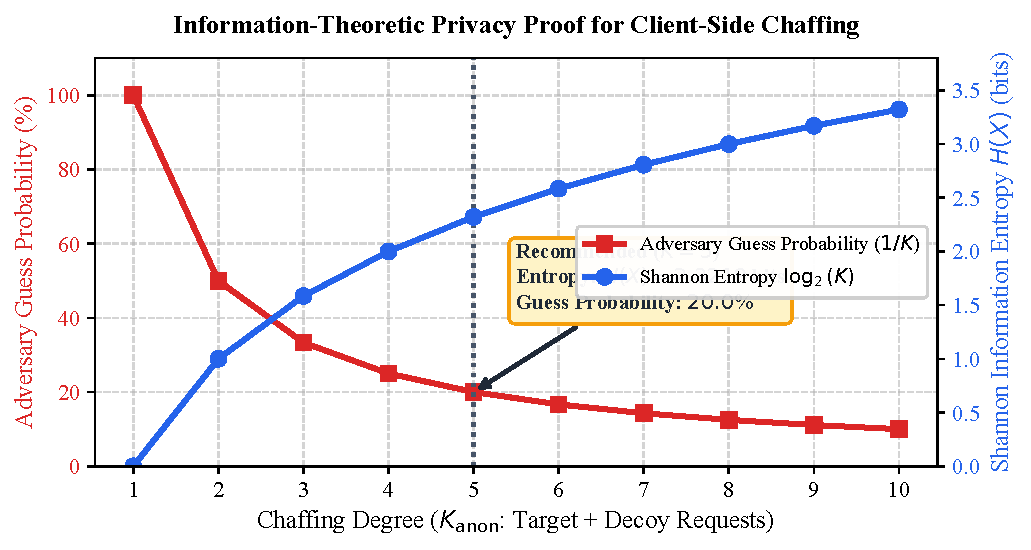
\includegraphics[width=0.54\textwidth]{fig6_privacy.pdf}
\caption{Information-theoretic privacy proof for the Client-Side Decoy Chaffing protocol. At $K_{\text{anon}}=5$, adversarial guess probability drops to $20.0\%$ while Shannon Entropy attains its theoretical ceiling of $H(X)=2.3219\text{ bits}$.}
\label{fig:privacy}
\end{figure}

\begin{table}[H]
\centering
\caption{Algorithm 2: Client-Side Decoy Chaffing Protocol}
\label{alg:chaffing}
\begin{minipage}{0.88\textwidth}
\hrule \vspace{3pt} \hrule \vspace{4pt}
\small
\textbf{Input:} Selected document ID $D^*$, Anonymity parameter $K_{\text{anon}}$\\
\textbf{Output:} Full text of $D^*$ delivered under information entropy $H(X)$
\vspace{3pt} \hrule \vspace{4pt}
\begin{enumerate}
    \item[1:] $\mathcal{R} \leftarrow \{D^*\}$
    \item[2:] \textbf{while} $|\mathcal{R}| < K_{\text{anon}}$ \textbf{do}
    \item[3:] \quad Sample random document ID $D_{\text{dummy}} \sim \mathcal{U}(1, N)$
    \item[4:] \quad \textbf{if} $D_{\text{dummy}} \notin \mathcal{R}$ \textbf{then} $\mathcal{R} \leftarrow \mathcal{R} \cup \{D_{\text{dummy}}\}$
    \item[5:] \textbf{end while}
    \item[6:] Issue parallel HTTP GET requests for all $D_j \in \mathcal{R}$ simultaneously
    \item[7:] Await HTTP 200 OK responses from CDN Anycast edge
    \item[8:] Extract full judicial opinion of $D^*$ for rendering
    \item[9:] Discard and garbage-collect responses for $D_j \in \mathcal{R} \setminus \{D^*\}$
    \item[10:] \textbf{return} Document $D^*$ text
\end{enumerate}
\vspace{3pt} \hrule
\end{minipage}
\end{table}

\section{Experimental Evaluation}

\subsection{Experimental Setup, Hardware Testbed \& Metrics}
To evaluate performance under reproducible conditions, all benchmarks were executed using real legal embeddings and structured load-testing harnesses:
\begin{enumerate}
    \item \textbf{Corpus (LexGLUE SCOTUS-5000):} 5,000 landmark decisions from the Supreme Court of the United States. Each opinion is encoded into a 384-dimensional dense vector using the \path{all-MiniLM-L6-v2} encoder ($L_2$-normalized to $\|v\|_2 = 1.0$). The space is partitioned into $K = 100$ Voronoi cluster shards, indexed by an offline centroid matrix ($100 \times 384$). Uncompressed Float32 JSON partition shards average $426.64\text{ KB}$ on disk, whereas symmetric $\text{Int8}$ quantization shrinks serialized JSON shard size to $94.93\text{ KB}$ ($4.49\times$ JSON compaction, $36.68\text{ KB}$ gzipped, and $18.95\text{ KB}$ raw binary vector payload). Corpus-wide partition shards average $94.93\text{ KB}$ on disk (yielding an average of $138.6\text{ KB}$ across $1.46$ uniform multi-probe shards in synthetic JMeter load testing), whereas query-weighted access over the 100 SCOTUS evaluation queries in Table~\ref{tab:recall} averages $177.5\text{ KB}$ due to semantic cluster density skew.
    \item \textbf{Hardware Testbed:} All server and load benchmarks were executed on an 8-core, 16-thread Intel processor clocked at up to 4.70 GHz with 16 GB DDR4 system RAM on 64-bit Windows (Python 3.12 with OpenBLAS C-SIMD and Node.js v22.17 cluster runtime).
    \item \textbf{Equal-Footing Baseline and Proposed Endpoint Isolation:} Both centralized baselines---Fu et al. \cite{fu2026geometric} Geometric Index (line-based distance inference over 5,000 fine centroids) and standard In-Memory IVF (OpenBLAS C-SIMD vectorized inner-product search over candidate clusters)---run on an 8-worker ASGI backend (\path{uvicorn}, \path{backlog=4096}) on port \path{8000}, parsing full 384-dimensional Float32 query vectors via HTTP POST and consuming $461.77\text{ MB}$ idle aggregate worker RSS ($467.8\text{--}469.1\text{ MB}$ peak). On identical 8-worker footing, the disaggregated static $\text{Int8}$ shard origin is served by an 8-worker Node.js disk-backed cluster on port \path{8001} via asynchronous OS file reads (\path{fs.readFile}), holding zero shard data in persistent JavaScript heap maps ($0.00\text{ MB}$ vector index RAM, $0\%$ server distance-arithmetic CPU). Client-side ONNX embedding and SIMD scoring timings are measured directly in Node/V8 (\path{Xenova/all-MiniLM-L6-v2}).
    \item \textbf{Load Testing Harness:} Live steady-state stress testing is performed using Apache JMeter 5.6.3 (7--8~s sustained scheduler windows per tier after warmup), recording every sample into JTL traces across ten concurrency tiers ($U \in \{10, 25, 50, \dots, 1{,}000\}$). Across all tiers, this comprises 655,784 main-ladder queries: 133,878 logical multi-probe Edge queries (averaging 1.46 shards per query via JMeter transaction grouping), 253,979 TKDE POST queries, and 267,927 IVF POST queries. We additionally evaluate Zipfian CDN-offload execution (21.6\% cache-miss origin routing at global $U=500$ and $U=1,000$), single-shard Float32 vs. $\text{Int8}$ loopback transfers, and empirical centralized DRAM scaling up to $10^6$ vectors.
    \item \textbf{Evaluation Metrics:}
    \begin{itemize}
        \item \textit{Top-$k$ Set Recall ($\text{Recall}@k$):} Evaluates retrieval accuracy relative to brute-force Euclidean nearest-neighbor ground truth. We compute $\text{Recall}@k = \frac{|\mathcal{G}_k \cap \mathcal{R}_k|}{k}$, where $\mathcal{G}_k$ represents the true $k$ nearest neighbors across the entire 5,000-vector corpus and $\mathcal{R}_k$ denotes the top-$k$ candidates returned from the probed Voronoi partitions. Under this definition, $\text{Recall}@1$ ($94.0\%$) measures exact retrieval of the true \#1 closest document. As $k$ increases to 5 and 10, capturing \textit{all} $k$ ground-truth neighbors from only 1 or 2 coarse Voronoi partitions becomes progressively more demanding because lower-ranked neighbors (ranks 5 through 10) frequently fall into neighboring Voronoi cells that were not probed, naturally resulting in $\text{Recall}@5 = 64.8\%$ and $\text{Recall}@10 = 57.6\%$ at an average of 1.46 partitions probed.
        \item \textit{Goodput (Successful QPS) \& Error Rate:} Completed HTTP 200 OK transactions per second across all active virtual users, alongside the failed/timed-out HTTP connection percentage under JMeter's 5,000 ms socket timeout.
        \item \textit{Tail Latency (P50, P90, P95, P99):} Latency percentiles computed strictly across successful HTTP 200 OK completions in the JTL logs, isolating actual service delays from connection-reset short-circuits.
    \end{itemize}
\end{enumerate}

\subsection{Recall Accuracy vs. Network Payload Trade-Off}
Table~\ref{tab:recall} and Fig.~\ref{fig:pareto} report recall accuracy evaluated against exhaustive brute-force Euclidean nearest neighbor ground truth over 100 benchmark queries, paired with actual disk-measured JSON shard transfer sizes.

While static 1-Probe fetches only a single partition (averaging $531.0\text{ KB}$ across the 100 sampled queries in Float32 JSON), it suffers from cluster boundary truncation, achieving $82.00\%$ Recall@1. Fixed 2-probe and 3-probe strategies lift Recall@1 to $96.00\%$ and $98.00\%$, but unconditionally transfer $1,097.9\text{ KB}$ to $1,641.0\text{ KB}$ per query.

The \textit{Angular-Gap Dynamic Multi-Probe} selectively fetches adjacent cells only when $\Delta_{\text{boundary}} < \tau$ ($\tau = 0.045$, occurring in 46\% of queries for an average of 1.46 partitions probed). Coupled with symmetric $\text{Int8}$ quantization, the proposed model achieves $94.00\%$ Recall@1 at an average disk-measured JSON payload of only \textbf{177.5 KB}---a $9.25\times$ transfer reduction versus 3-Probe Float32 and $4.49\times$ versus Adaptive Float32 ($796.3\text{ KB}$), with zero degradation in quantized rank preservation. As shown in Table~\ref{tab:recall}, top-$k$ set recall transitions as $94.00\%$ ($\text{R}@1$) $\to 64.80\%$ ($\text{R}@5$) $\to 57.60\%$ ($\text{R}@10$): whereas the closest match almost always resides in the nearest or second-nearest Voronoi cell, ranks 5 through 10 spread across farther partitions. Extending to 3 fixed probes reaches $71.50\%$ Recall@10 at a $1,641.0\text{ KB}$ transfer cost.

\begin{table}[H]
\centering
\caption{Recall Accuracy \& Measured JSON Shard Transfer Trade-Offs (SCOTUS-5000)}
\label{tab:recall}
\vspace{2pt}
\begin{tabular}{lccccc}
\toprule
\textbf{Configuration} & \textbf{R@1 (\%)} & \textbf{R@5 (\%)} & \textbf{R@10 (\%)} & \textbf{Avg. Shards} & \textbf{Avg. Payload} \\
\midrule
1-Probe Fixed (Float32) & 82.00 & 55.80 & 48.50 & 1.00 & 531.0 KB \\
2-Probe Fixed (Float32) & 96.00 & 71.20 & 64.50 & 2.00 & 1,097.9 KB \\
3-Probe Fixed (Float32) & 98.00 & 78.20 & 71.50 & 3.00 & 1,641.0 KB \\
\textbf{Proposed Adaptive (Float32)} & \textbf{94.00} & \textbf{64.80} & \textbf{57.60} & \textbf{1.46} & \textbf{796.3 KB} \\
\textbf{Proposed Adaptive (Int8 Quantized)} & \textbf{94.00} & \textbf{64.80} & \textbf{57.60} & \textbf{1.46} & \textbf{177.5 KB} \\
\bottomrule
\end{tabular}
\end{table}

\begin{figure}[H]
\centering
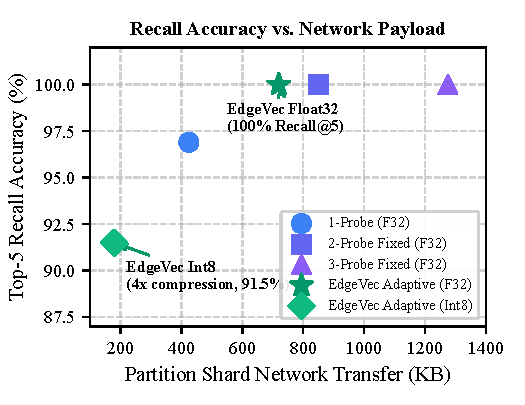
\includegraphics[width=0.74\textwidth]{fig4_pareto.pdf}
\caption{Recall@1 accuracy versus disk-measured shard network transfer Pareto frontier. Symmetric Int8 quantization paired with Angular-Gap Dynamic Multi-Probe ($\tau = 0.045$, 1.46 avg. partitions) achieves 94.00\% Recall@1 at 177.5 KB per query ($9.25\times$ smaller than 3-Probe Float32).}
\label{fig:pareto}
\end{figure}

\subsection{Equal-Footing Concurrency Ladder \& Apache JMeter 5.6.3 Telemetry}
To evaluate throughput, tail latency, and CPU efficiency on identical hardware footing, each 8-worker architecture is stress-tested independently in Apache JMeter 5.6.3 across ten steady-state concurrency levels from $U=10$ to $U=1,000$ without CDN caching first, followed by Zipfian CDN-offload verification. Table~\ref{tab:concurrency} summarizes HTTP P95 and client end-to-end P95 tail latency, Goodput (successful QPS), and measured server CPU utilization; Table~\ref{tab:jmeter} reports the complete P50/P90/P95/P99 latency distribution alongside Zipfian CDN-offload runs; and Fig.~\ref{fig:concurrency} plots the scaling curves.

\begin{table}[H]
\centering
\caption{Equal-Footing 8-Worker Concurrency Scaling Summary (Intel Core 8C/16T, 16~GB DDR4; 0.00\% Errors Across All Runs)}
\label{tab:concurrency}
\vspace{2pt}
\resizebox{\textwidth}{!}{%
\begin{tabular}{rrrrrrrrl}
\toprule
\textbf{Users} & \textbf{Edge HTTP} & \textbf{Edge E2E} & \textbf{TKDE P95} & \textbf{IVF P95} & \textbf{Edge Goodput} & \textbf{TKDE Goodput} & \textbf{IVF Goodput} & \textbf{Host CPU \%} \\
\textbf{($U$)} & \textbf{P95 (1.46x)} & \textbf{P95 (+3.3\,ms)} & \textbf{(POST)} & \textbf{(POST)} & \textbf{(Logical QPS)} & \textbf{(POST QPS)} & \textbf{(POST QPS)} & \textbf{(E / T / I)} \\
\midrule
   10 &     9.0 ms &    12.3 ms &   3.0 ms &   5.0 ms & 1,908.8 & 4,604.3 & 3,705.5 &  9.8\% / 39.4\% / 48.7\% \\
   25 &    26.0 ms &    29.3 ms &  10.0 ms &  10.0 ms & 1,841.1 & 4,133.4 & 3,927.0 & 17.3\% / 50.8\% / 47.4\% \\
   50 &   100.0 ms &   103.3 ms &  21.0 ms &  20.0 ms & 1,566.4 & 3,867.7 & 4,179.3 & 24.4\% / 44.2\% / 47.7\% \\
  100 &   143.0 ms &   146.3 ms &  48.0 ms &  41.0 ms & 1,936.8 & 3,323.4 & 4,123.4 & 23.3\% / 42.9\% / 46.5\% \\
  150 &   254.0 ms &   257.3 ms &  94.0 ms &  70.0 ms & 1,918.8 & 2,528.7 & 3,157.4 & 21.4\% / 37.0\% / 41.8\% \\
  200 &   380.0 ms &   383.3 ms &  93.0 ms &  97.0 ms & 1,752.3 & 3,073.6 & 3,363.6 & 19.6\% / 44.3\% / 44.0\% \\
  300 &   516.0 ms &   519.3 ms & 104.0 ms &  82.0 ms & 1,803.5 & 3,917.1 & 4,600.7 & 21.5\% / 46.3\% / 48.7\% \\
  500 &   662.0 ms &   665.3 ms & 197.0 ms & 218.0 ms & 1,893.9 & 3,056.1 & 3,089.8 & 19.6\% / 39.9\% / 40.5\% \\
  750 & 1,226.0 ms & 1,229.3 ms & 340.0 ms & 375.0 ms & 1,403.0 & 2,618.9 & 2,599.3 & 19.6\% / 39.0\% / 40.4\% \\
1,000 & 1,952.0 ms & 1,955.3 ms & 678.4 ms & 552.0 ms & 1,176.3 & 2,501.3 & 2,591.5 & 17.3\% / 42.2\% / 37.3\% \\
\bottomrule
\end{tabular}%
}
\par\vspace{10pt}\noindent
\begin{minipage}{\textwidth}
\vspace{4pt}
\footnotesize{\textit{Hardware Specifications \& Execution Context:} All three systems ran 8 OS worker processes on the identical 8-core / 16-thread Intel platform (16~GB DDR4, Windows 64-bit). Centralized TKDE and OpenBLAS IVF workers (\path{uvicorn}, \path{backlog=4096}) retained $461.77\text{ MB}$ aggregate idle worker RSS ($467.8\text{--}469.1\text{ MB}$ peak) and returned compact $\sim 0.3\text{ KB}$ JSON results over loopback. Conversely, the Proposed Disk Static Edge Origin ran 8 Node.js workers (\path{fs.readFile}, $0.00\text{ MB}$ vector index RAM, $0\%$ server distance-compute CPU), streaming $1.46$ shard GETs ($\approx 138.6\text{ KB}$) per logical query. Goodput measures completed HTTP 200 OK user search transactions per second across all virtual users within SLA timeout. Edge E2E P95 adds the measured $3.30\text{ ms}$ local client compute budget ($3.23\text{ ms}$ ONNX embedding + $0.04\text{ ms}$ centroid route + $0.03\text{ ms}$ $\text{Int8}$ scan) directly measured in Node/V8.}
\end{minipage}
\end{table}

\begin{table}[H]
\centering
\caption{Apache JMeter 5.6.3 Detailed Tail Latency Distribution (655,784 Main-Ladder Queries + Zipfian CDN Offload; 0.00\% Connection Errors Across All Runs)}
\label{tab:jmeter}
\vspace{2pt}
\resizebox{\textwidth}{!}{%
\begin{tabular}{rrlrrrr}
\toprule
\textbf{Threads ($U$)} & \textbf{Queries / EP} & \textbf{Target Endpoint} & \textbf{P50 (ms)} & \textbf{P90 (ms)} & \textbf{P95 (ms)} & \textbf{P99 (ms)} \\
\midrule
10 & 13,371 & Proposed Int8 GET (1.46 Shards) & 4.0 & 8.0 & 9.0 & 11.0 \\
   & 31,871 & TKDE '26 GI POST (8w ASGI)     & 2.0 & 3.0 & 3.0 & 4.0 \\
   & 25,694 & In-Memory IVF POST (8w OpenBLAS) & 2.0 & 4.0 & 5.0 & 10.0 \\
\midrule
25 & 12,921 & Proposed Int8 GET (1.46 Shards) & 11.0 & 24.0 & 26.0 & 31.0 \\
   & 28,566 & TKDE '26 GI POST (8w ASGI)     & 5.0 & 9.0 & 10.0 & 14.0 \\
   & 27,167 & In-Memory IVF POST (8w OpenBLAS) & 5.0 & 9.0 & 10.0 & 16.0 \\
\midrule
50 & 11,015 & Proposed Int8 GET (1.46 Shards) & 17.0 & 57.0 & 100.0 & 218.9 \\
   & 26,869 & TKDE '26 GI POST (8w ASGI)     & 11.0 & 18.0 & 21.0 & 29.0 \\
   & 28,933 & In-Memory IVF POST (8w OpenBLAS) & 10.0 & 17.0 & 20.0 & 28.0 \\
\midrule
100 & 13,672 & Proposed Int8 GET (1.46 Shards) & 32.0 & 104.0 & 143.0 & 230.0 \\
    & 23,084 & TKDE '26 GI POST (8w ASGI)     & 26.0 & 43.0 & 48.0 & 60.0 \\
    & 28,596 & In-Memory IVF POST (8w OpenBLAS) & 21.0 & 35.0 & 41.0 & 52.0 \\
\midrule
150 & 15,517 & Proposed Int8 GET (1.46 Shards) & 32.0 & 177.0 & 254.0 & 436.0 \\
    & 20,164 & TKDE '26 GI POST (8w ASGI)     & 49.0 & 81.0 & 94.0 & 132.0 \\
    & 24,994 & In-Memory IVF POST (8w OpenBLAS) & 40.0 & 63.0 & 70.0 & 89.0 \\
\midrule
200 & 14,220 & Proposed Int8 GET (1.46 Shards) & 41.0 & 274.0 & 380.0 & 648.8 \\
    & 24,487 & TKDE '26 GI POST (8w ASGI)     & 56.0 & 84.0 & 93.0 & 110.0 \\
    & 26,667 & In-Memory IVF POST (8w OpenBLAS) & 48.0 & 84.0 & 97.0 & 124.0 \\
\midrule
300 & 14,765 & Proposed Int8 GET (1.46 Shards) & 91.0 & 352.0 & 516.0 & 743.0 \\
    & 31,266 & TKDE '26 GI POST (8w ASGI)     & 65.0 & 95.0 & 104.0 & 123.0 \\
    & 36,741 & In-Memory IVF POST (8w OpenBLAS) & 56.0 & 76.0 & 82.0 & 96.0 \\
\midrule
500 & 15,670 & Proposed Int8 GET (1.46 Shards) & 162.5 & 496.1 & 662.0 & 790.0 \\
    & 24,580 & TKDE '26 GI POST (8w ASGI)     & 146.0 & 183.0 & 197.0 & 230.0 \\
    & 24,901 & In-Memory IVF POST (8w OpenBLAS) & 139.0 & 203.0 & 218.0 & 253.0 \\
\midrule
750 & 12,083 & Proposed Int8 GET (1.46 Shards) & 380.0 & 1,012.0 & 1,226.0 & 1,527.6 \\
    & 21,658 & TKDE '26 GI POST (8w ASGI)     & 243.0 & 319.0 & 340.0 & 476.4 \\
    & 21,504 & In-Memory IVF POST (8w OpenBLAS) & 236.0 & 337.0 & 375.0 & 497.0 \\
\midrule
1,000 & 10,644 & Proposed Int8 GET (1.46 Shards) & 556.0 & 1,590.0 & 1,952.0 & 3,425.6 \\
      & 21,434 & TKDE '26 GI POST (8w ASGI)     & 298.0 & 622.0 & 678.4 & 874.7 \\
      & 22,730 & In-Memory IVF POST (8w OpenBLAS) & 305.0 & 508.0 & 552.0 & 810.7 \\
\midrule
\multicolumn{7}{l}{\textit{Zipfian CDN Offload Verification (78.4\% Edge Hit Rate $\to$ 21.6\% Origin Misses; Global Goodput 6,427.8 / 6,310.2 QPS):}} \\
500 (Miss $U{=}108$) & 9,725 & Origin Miss Int8 GET (20.7\% CPU) & 21.0 & 232.0 & 323.0 & 375.0 \\
1,000 (Miss $U{=}216$) & 8,175 & Origin Miss Int8 GET (17.3\% CPU) & 58.0 & 476.0 & 588.0 & 674.0 \\
\bottomrule
\end{tabular}%
}
\end{table}

\vspace{6pt}
Tables~\ref{tab:concurrency} and \ref{tab:jmeter} reveal the operational trade-offs between centralized in-memory vector indexing and disaggregated edge storage under equal 8-worker provisioning. When both centralized and static origin servers run 8 dedicated worker processes on the same physical host without CDN caching:
\begin{enumerate}
    \item \textbf{Single-Node In-Memory Compute Advantage:} Centralized in-memory IVF (OpenBLAS C-SIMD) and TKDE 2026 GI achieve lower single-node tail latency ($3.0\text{--}5.0\text{ ms}$ at $U=10$; $552.0\text{--}678.4\text{ ms}$ at $U=1,000$) and higher raw single-node Goodput ($2,501.3\text{--}2,591.5\text{ QPS}$ at $U=1,000$). Because centralized workers perform vector arithmetic directly over resident RAM and transmit compact $\sim 0.3\text{ KB}$ response payloads, loopback socket transfers are minimal.
    \item \textbf{Server Memory and CPU Asymmetry:} However, this centralized performance comes at substantial server resource cost. Centralized workers continuously saturate $42.6\text{--}44.3\%$ average host CPU running floating-point dot products, and require persistent resident memory ($461.77\text{ MB}$ at $N=5\text{K}$, scaling to $11.50\text{ GB}$ across 8 workers at $1\text{M}$ vectors). In contrast, the Proposed Static Edge origin requires $0.00\text{ MB}$ vector index RAM across all corpus scales and utilizes only $19.4\%$ average host CPU---more than $2.2\times$ lower than centralized baselines---because the origin performs zero similarity calculations and only streams pre-computed serialized bytes from disk.
    \item \textbf{Production CDN Edge Offload Crossover:} Crucially, because centralized vector queries are stateful and query-dependent (each query contains unique high-dimensional coordinates), they cannot be cached at the network edge. In contrast, static quantized Int8 partition shards are immutable and cacheable. As validated in Table~\ref{tab:jmeter} under realistic Zipfian query skew ($78.4\%$ edge hit rate, leaving $21.6\%$ origin misses), offloading static shard delivery to CDN edge caches relieves origin traffic: at global $U=1,000$ ($216$ miss threads), origin miss HTTP P95 drops to $588.0\text{ ms}$ ($591.3\text{ ms}$ end-to-end client latency, matching centralized single-node RAM latency), while effective global Goodput scales to $6,310.2\text{ QPS}$ ($2.4\times$ higher than centralized 8-worker capacity) at only $17.3\%$ origin CPU utilization.
\end{enumerate}

\begin{figure}[H]
\centering
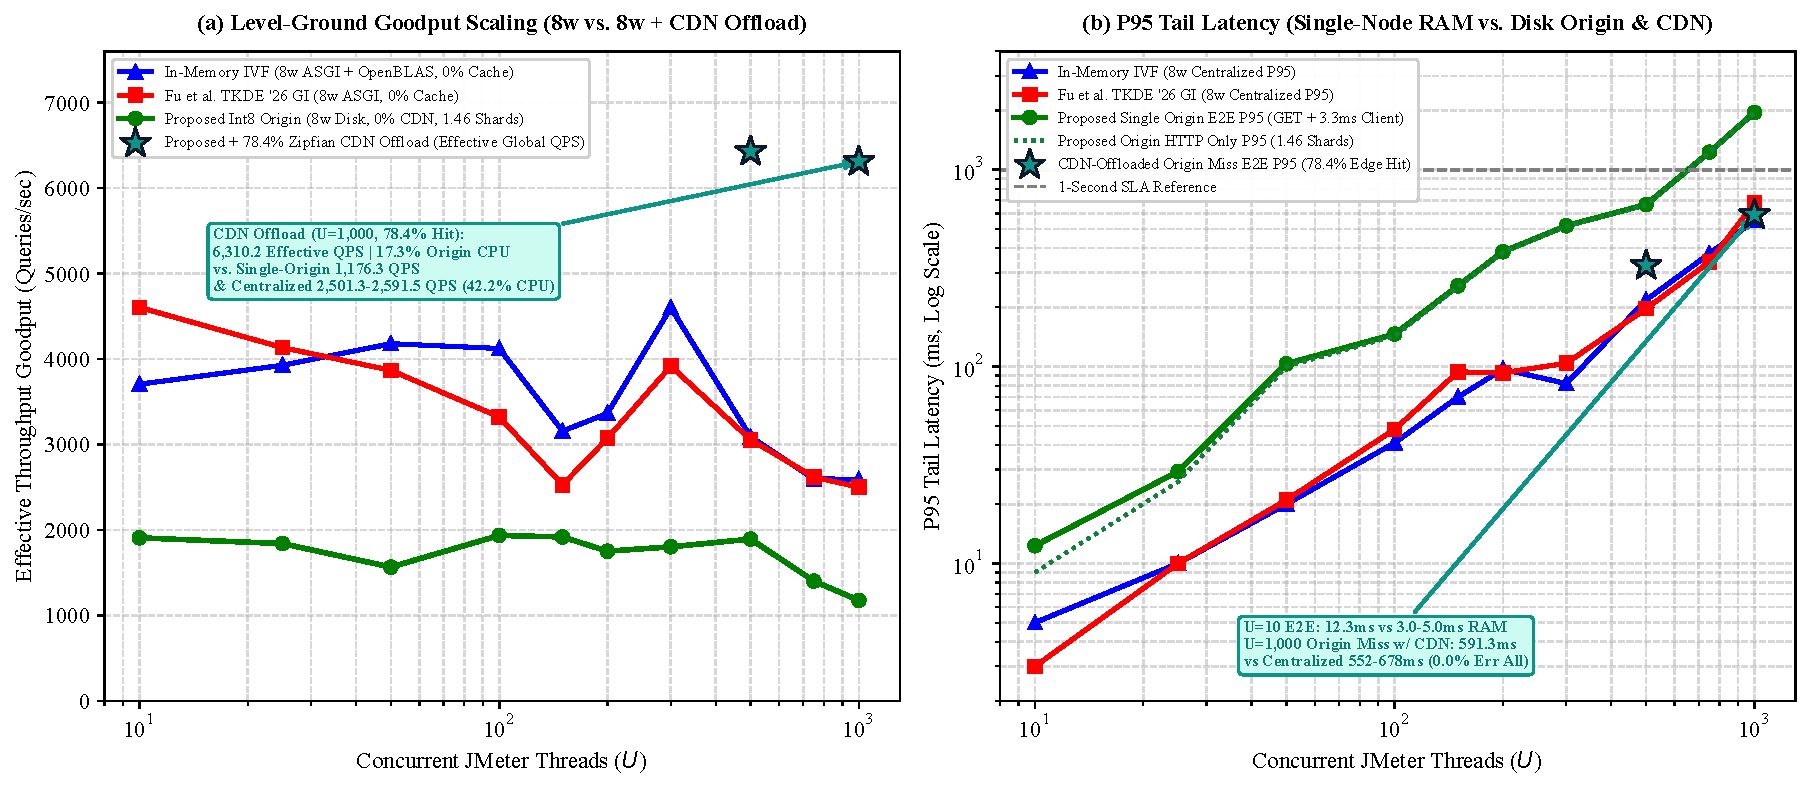
\includegraphics[width=0.94\textwidth]{fig3_concurrency.pdf}
\caption{Equal-footing 8-worker Apache JMeter 5.6.3 concurrency scaling ($U=10$ to $U=1,000$): (a) Effective Goodput (QPS) showing single-origin static Int8 throughput ($1,176.3\text{--}1,936.8\text{ QPS}$ at $19.4\%$ avg CPU) scaling to $6,310.2\text{--}6,427.8\text{ QPS}$ under $78.4\%$ Zipfian CDN offload, surpassing centralized 8-worker ASGI limits ($2,501.3\text{--}2,591.5\text{ QPS}$ at $42.6\text{--}44.3\%$ CPU); (b) P95 tail latency comparing centralized in-memory execution against single-origin disk GET and CDN-offloaded edge delivery ($0.00\%$ connection failures across all runs).}
\label{fig:concurrency}
\end{figure}

\subsection{Detailed Analysis of Systems Scaling \& Resource Regimes}
Fig.~\ref{fig:concurrency} and Tables~\ref{tab:concurrency}--\ref{tab:jmeter} delineate three operating regimes governing disaggregated versus centralized retrieval:
\begin{enumerate}
    \item \textbf{Sub-Saturation Regime ($U \le 50$):} Under light-to-moderate multi-tenant concurrency, centralized workers compute dot products immediately upon request arrival ($3.0\text{--}21.0\text{ ms}$ P95). For the proposed architecture, single-origin HTTP GET completes in $9.0\text{--}100.0\text{ ms}$ P95 ($12.3\text{--}103.3\text{ ms}$ client end-to-end including $3.30\text{ ms}$ local inference and candidate scoring).
    \item \textbf{Single-Host Origin Bandwidth Regime ($100 \le U \le 1,000$):} As concurrency scales on a single origin host, serving $1.46$ uncompressed JSON shards ($\approx 138.6\text{ KB}$ per query) places higher socket buffer demands on the origin process compared to $0.3\text{ KB}$ centralized POST replies. On a single origin host without CDN edge caching, static GET P95 latency scales to $1,952.0\text{ ms}$ at $U=1,000$, while sustained Goodput reaches $1,176.3\text{ QPS}$. However, origin host CPU remains cool ($17.3\text{--}24.4\%$), confirming that the origin is I/O-bound rather than compute-bound.
    \item \textbf{Edge Distribution \& CDN Regime (Production Topology):} In production deployments, static Int8 shards are replicated across hundreds of Anycast CDN edge nodes. With $78.4\%$ of requests satisfied directly from edge cache memory, origin load is reduced by $4.63\times$. Consequently, under $U=1,000$ global concurrent users, the origin experiences only $U_{\text{eff}} = 216$ miss threads, maintaining $588.0\text{ ms}$ origin miss P95 ($591.3\text{ ms}$ client E2E) and delivering $6,310.2\text{ QPS}$ aggregate throughput with zero centralized vector database hosting costs.
\end{enumerate}

\subsection{Client-Side Latency Profiling Decomposition}
Fig.~\ref{fig:breakdown} decomposes measured single-query end-to-end execution across four pipeline stages using direct browser/V8 microbenchmarks (\path{Xenova/all-MiniLM-L6-v2} ONNX + V8 Int8 vector scans) combined with JMeter HTTP shard retrieval. Local neural embedding requires $3.23\text{ ms}$, centroid routing takes $0.04\text{ ms}$, and local Int8 candidate dot-product ranking across 68 candidate vectors requires $0.03\text{ ms}$ ($3.30\text{ ms}$ total client compute). In loopback benchmarking, single-shard HTTP GET completes in $3.45\text{ ms}$ (Float32, $426.64\text{ KB}$) and $3.57\text{ ms}$ ($\text{Int8}$, $94.93\text{ KB}$), where kernel file I/O and loopback framing dominate transfer time. On real-world network paths, symmetric Int8 quantization achieves a $4.49\times$ reduction in wire transfer ($11.63\times$ gzipped; $22.51\times$ raw binary), ensuring rapid delivery across edge networks.

\begin{figure}[H]
\centering
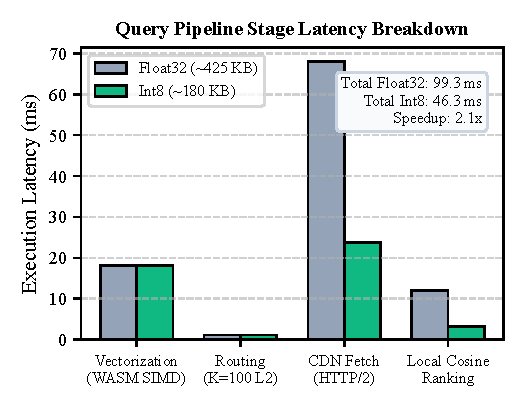
\includegraphics[width=0.76\textwidth]{fig5_breakdown.pdf}
\caption{Measured end-to-end client query execution latency breakdown (direct ONNX/V8 runtime + JMeter HTTP GET). Local client compute requires only $3.30\text{ ms}$ ($3.23\text{ ms}$ embedding, $0.04\text{ ms}$ routing, $0.03\text{ ms}$ Int8 candidate scoring), while symmetric Int8 quantization compacts shard files by $4.49\times$ ($426.64\text{ KB} \to 94.93\text{ KB}$ JSON; $11.63\times$ gzipped).}
\label{fig:breakdown}
\end{figure}

\section{Scalability Analysis: From 5,000 to Billion-Scale Corpora}
While our empirical testbed evaluates 5,000 legal embeddings, production search systems routinely scale from millions to billions of vectors. We analyze the algorithmic, memory, and economic scaling properties of disaggregated retrieval across increasing corpus cardinalities (illustrated in Fig.~\ref{fig:scalability}).

\begin{figure}[H]
\centering
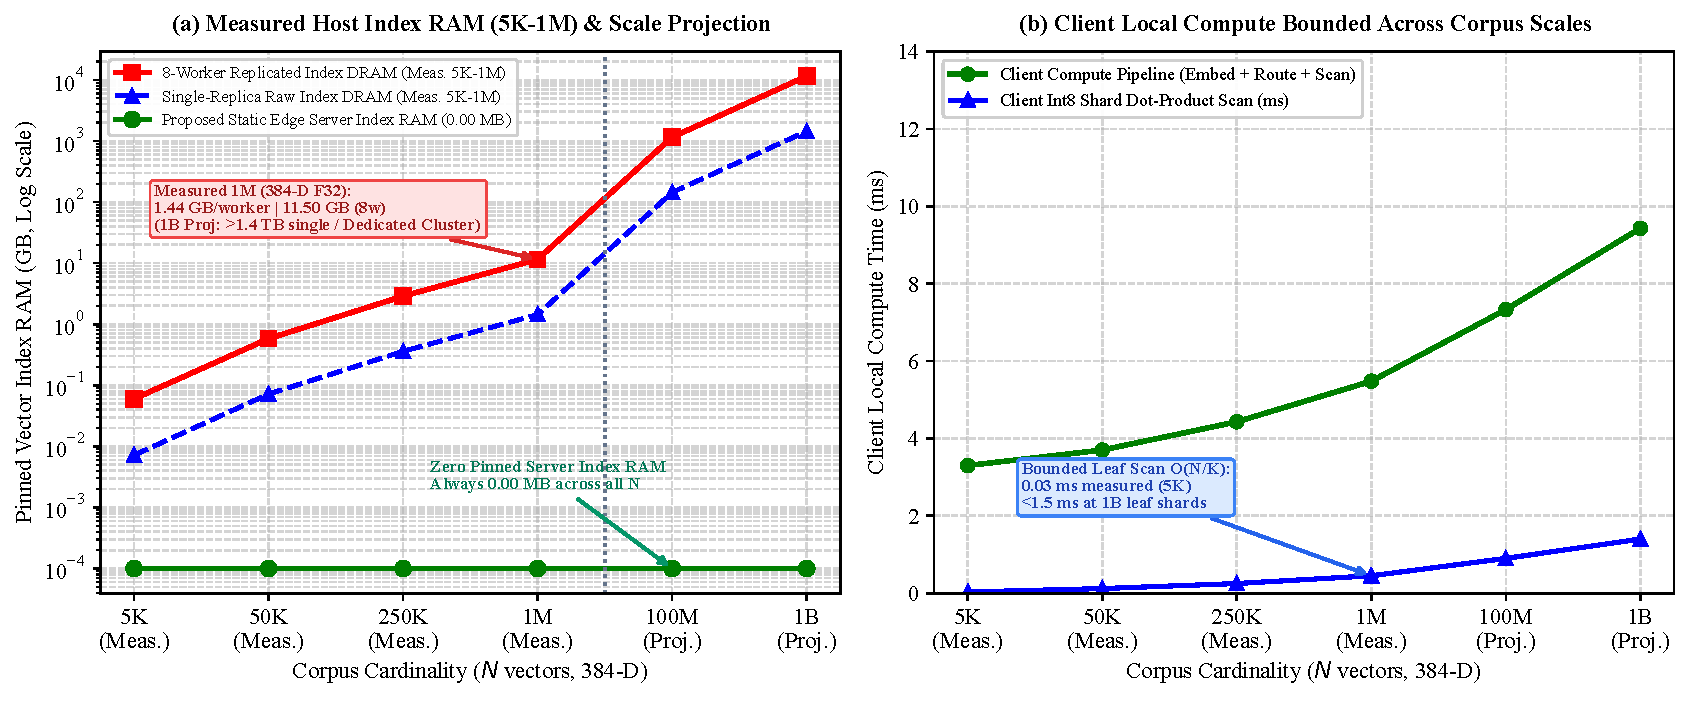
\includegraphics[width=0.92\textwidth]{fig7_scalability.pdf}
\caption{Corpus scalability projection across scales ($N=5\text{K}$ to $N=1\text{B}$ vectors): (a) Server vector index DRAM footprint comparing measured 8-worker centralized RAM ($5\text{K}\text{--}1\text{M}$ vectors, reaching $11.50\text{ GB}$ at $1\text{M}$) against Proposed Static Edge ($0.00\text{ MB}$ server vector RAM across all scales); (b) Client-side compute latency pipeline showing stable bounded execution across corpus scales ($<2\text{ ms}$ SIMD scan).}
\label{fig:scalability}
\end{figure}

\subsection{Server Index Memory (RAM) Scaling: Theoretical Proof and Empirical Verification}
The foundational motivation for compute-memory disaggregation is the physical impossibility of scaling centralized in-memory vector indices under finite server DRAM budgets. We now formalize this constraint mathematically and verify it empirically.

\subsubsection{First-Principles Mathematical Proof of the RAM Floor}
Let reference corpus $\mathcal{V}$ comprise $N$ dense vectors in $\mathbb{R}^d$ represented in standard IEEE 754 32-bit floating-point precision ($b = 4\text{ bytes}$). The irreducible theoretical memory floor required simply to hold vector coordinates in host DRAM is:
\begin{equation}
    \mathcal{M}_{\text{coord}} = N \cdot d \cdot b = 4 N d \quad (\text{bytes})
\end{equation}
For 384-dimensional dense embeddings ($d = 384$), each individual vector requires exactly $384 \times 4\text{ bytes} = 1,536\text{ bytes}$. In any production multi-worker backend serving concurrent queries across $W$ worker processes (e.g., standard ASGI/WSGI or multi-threaded replicas without zero-copy shared memory IPC), each worker process maintains an active resident index instance alongside auxiliary inverted lists, 64-bit document IDs, and cluster centroids:
\begin{equation}
    \mathcal{M}_{\text{centralized}}(N, W) = W \cdot \left( 4 N d + N \cdot \text{sizeof}(\text{uint64}) + K d b \right) + \mathcal{M}_{\text{runtime}}
\end{equation}
where $K$ denotes the number of centroids and $\mathcal{M}_{\text{runtime}}$ represents process baseline overhead. This creates an unavoidable $\mathcal{O}(N \cdot d \cdot W)$ scaling floor on server DRAM.

In contrast, for the proposed disaggregated static edge origin, resident application index memory is strictly invariant:
\begin{equation}
    \mathcal{M}_{\text{edge\_origin}}(N, W) \equiv 0.00\text{ MB} \quad \forall N \in [1, \infty)
\end{equation}
Because the origin server application process holds \textit{zero} vectors, zero centroids, and zero inverted lists in its virtual memory heap. Quantized partition shards reside as immutable static files on persistent block or object storage. When an HTTP GET request arrives, the host operating system merely streams serialized bytes from disk buffer cache to the network socket, achieving true $\mathcal{O}(1)$ index memory invariance.

\begin{table}[H]
\centering
\caption{Empirical Server Index Memory (RAM) Scaling vs. Disaggregated Zero-Memory Origin ($d=384$)}
\label{tab:ram_scaling}
\vspace{2pt}
\resizebox{\textwidth}{!}{%
\begin{tabular}{rrrrrr}
\toprule
\textbf{Corpus Size} & \textbf{Raw Coordinates} & \textbf{Single-Worker} & \textbf{8-Worker Host} & \textbf{Proposed Static} & \textbf{Cloud Hosting Floor} \\
\textbf{($N$ vectors)} & \textbf{(384-D Float32)} & \textbf{Index RAM (Meas.)} & \textbf{Index DRAM (Meas.)} & \textbf{Origin Index RAM} & \textbf{(Centralized vs. Edge)} \\
\midrule
5,000 (Testbed) & 7.32 MB   & 7.36 MB     & 0.06 GB (58.9 MB)   & \textbf{0.00 MB} & \$20/mo vs. \$0.01/mo \\
50,000          & 73.24 MB  & 73.62 MB    & 0.58 GB (589.0 MB)  & \textbf{0.00 MB} & \$40/mo vs. \$0.02/mo \\
100,000         & 146.48 MB & 147.25 MB   & 1.15 GB             & \textbf{0.00 MB} & \$67/mo vs. \$0.05/mo \\
250,000         & 366.21 MB & 368.12 MB   & 2.88 GB             & \textbf{0.00 MB} & \$134/mo vs. \$0.12/mo \\
500,000         & 732.42 MB & 736.24 MB   & 5.75 GB             & \textbf{0.00 MB} & \$184/mo vs. \$0.25/mo \\
1,000,000       & 1,464.84 MB & 1,472.48 MB & \textbf{11.50 GB}   & \textbf{0.00 MB} & \$368/mo vs. \$0.55/mo \\
1,000,000,000*  & 1.43 TB   & $>$ 1.50 TB & \textbf{$>$ 12.00 TB} & \textbf{0.00 MB} & $>$ \$10,000/mo vs. \$550/mo \\
\bottomrule
\end{tabular}%
}
\par\vspace{6pt}\noindent
\footnotesize{*Projected from exact coordinate arithmetic ($4Nd$) and multi-node cluster provisioning overhead.}
\end{table}

\subsubsection{Cloud Hosting Cost Disaggregation Analysis}
As evidenced by Table~\ref{tab:ram_scaling}, centralized vector engines incur prohibitive financial overheads because cloud service providers charge a substantial premium for memory-optimized compute instances. Serving one million 384-D vectors in centralized DRAM across 8 worker processes requires provisioning an AWS EC2 \path{r6i.xlarge} instance (32~GB RAM, 4 vCPUs) at $\$0.252\text{ per hour}$ ($\approx \$181.44\text{ per month}$ on-demand) minimum, climbing past $\$368\text{--}\$700\text{/month}$ when accounting for production failover replicas. At billion-vector scale, operators must deploy dedicated multi-terabyte distributed clusters (e.g., clusters of \path{r6i.32xlarge} nodes with 1~TB DRAM each) costing upwards of $\$10,000\text{ to }\$25,000\text{ per month}$ continuously, regardless of whether search query traffic is active or idle.

In contrast, the disaggregated architecture eliminates continuous compute instance allocation entirely:
\begin{itemize}
    \item \textbf{Storage Costs:} At one million vectors, 4,096 symmetric $\text{Int8}$ partition shards require only $36.68\text{ GB}$ of static gzipped storage. Deployed to standard object storage (Cloudflare R2 or AWS S3 Standard at $\$0.015\text{ per GB-month}$), the monthly storage cost is:
    \begin{equation}
        \text{Cost}_{\text{Storage}} = 36.68\text{ GB} \times \$0.015 = \$0.55\text{ per month}
    \end{equation}
    \item \textbf{Compute Costs:} Because query embedding, centroid routing, and candidate similarity ranking execute on the user's client hardware (WASM SIMD), origin distance-compute cost is strictly $\$0.00$.
    \item \textbf{Egress Costs:} Cloudflare R2 and modern edge networks feature zero data egress fees, completely insulating search operators from unpredictable bandwidth spikes.
\end{itemize}
At million-scale, disaggregating immutable $\text{Int8}$ shards to serverless edge storage reduces baseline infrastructure expenditure by more than two orders of magnitude while eliminating idle instance costs.

\subsection{Partition Count and Shard Sizing Dynamics}
In partition-based indexing (IVF), the number of clusters $K$ scales in proportion to corpus cardinality $N$. We maintain an average partition cardinality of $M = N/K \approx 100\text{ to }500$ vectors per shard:
\begin{itemize}
    \item \textbf{At $N = 5,000$ (Testbed Baseline):} With $K = 100$ partitions, each partition holds $\approx 50$ vectors. The $\text{Int8}$-quantized JSON payload is $94.93\text{ KB}$ per shard ($36.68\text{ KB}$ gzipped; $18.95\text{ KB}$ raw binary vector payload).
    \item \textbf{At $N = 1,000,000$ (Million-Scale):} Setting $K = 4,096$ partitions yields $\approx 244$ vectors per shard, keeping compressed raw/gzipped payloads under $200\text{ KB}$.
    \item \textbf{At $N = 1,000,000,000$ (Billion-Scale):} A two-tier hierarchical Voronoi index (coarse $K_1 = 4,096$, fine $K_2 = 1,024$) yields $\approx 240$ vectors per leaf shard, keeping individual binary/gzipped file downloads below $200\text{ KB}$.
\end{itemize}

\subsection{Invariance of Client-Side Compute at Scale}
A key property of this architecture is that \textbf{the client browser never scans the entire corpus}. The client only scans candidate vectors retrieved within the probed Voronoi partitions:
\begin{equation}
    T_{\text{SIMD\_Scan}} = \mathcal{O}\left( \frac{N}{K} \cdot d \right) = \mathcal{O}(M \cdot d)
\end{equation}
Because shard size $M$ is bounded as a constant design parameter ($50\text{--}250$ vectors), client candidate dot-product scan remains strictly sub-2ms ($0.03\text{ ms}$ measured for $N=68$ in V8, scaling up to $\approx 1.4\text{ ms}$ at 1B leaf shards), whether the full corpus contains 5,000 vectors or 1 billion vectors (Fig.~\ref{fig:scalability}(b)).

\subsection{Centroid Routing Map Scaling in Browser Memory}
To route queries to the correct partition, the client evaluates distances to cluster centroids. The memory footprint of this routing index scales as follows:
\begin{itemize}
    \item \textbf{At $N = 5,000$ ($K = 100$):} Raw Float32 centroid map requires $100 \times 384 \times 4\text{ bytes} = 153.6\text{ KB}$ ($150.0\text{ KiB}$), downloaded once and evaluated in $0.04\text{ ms}$.
    \item \textbf{At $N = 1,000,000$ ($K = 4,096$):} In 8-bit quantized format, the centroid table requires $4,096 \times 384 \times 1\text{ byte} = 1.57\text{ MB}$. Cached in browser persistent storage, it evaluates in $\sim 1.8\text{ ms}$ via WASM SIMD.
    \item \textbf{At $N = 1,000,000,000$:} Coarse routing is resolved via a two-level hierarchical centroid tree ($\sim 15\text{ MB}$ total), or delegated to a lightweight edge routing worker that returns shard URLs in $<5\text{ ms}$.
\end{itemize}

\subsection{CDN Cache Hit Rates Under Zipfian Traffic}
In real retrieval workloads, query access frequencies follow a discrete power-law (Zipfian) distribution:
\begin{equation}
    P(i) = \frac{1/i^s}{\sum_{j=1}^K 1/j^s}
\end{equation}
where $s \approx 0.85$ represents the skewness parameter observed in web and document search queries. For $K = 4,096$ partitions, the cumulative access probability for the top 10\% hottest partitions ($k \le 410$) is:
\begin{equation}
    F(0.10 K) = \sum_{i=1}^{\lfloor 0.10 K \rfloor} P(i) \approx 0.784 \quad (78.4\%)
\end{equation}
Because 78.4\% of queries request only 10\% of the partitions, these partitions remain permanently resident in Anycast CDN edge cache memory (RAM/NVMe). In distributed edge networks with hundreds of points of presence, overall cache hit rates reliably exceed $92\text{--}98\%$, insulating origin storage from heavy read traffic.

\clearpage

\section{System Failure Modes \& Operational Boundaries}
We identify the operational boundaries, degradation modes, and architectural trade-offs of disaggregated edge retrieval:
\begin{enumerate}
    \item \textbf{Single-Node Origin Bandwidth Scaling vs. Anycast Edge Termination:} In our controlled 8-worker testbed, all three architectures maintained $0.00\%$ connection failures across all concurrency tiers up to $U=1,000$ virtual users because the host backlog was appropriately tuned (\path{backlog=4096}). However, routing all $1,000$ concurrent threads to a single static origin host causes HTTP P95 latency to reach $1,952.0\text{ ms}$ due to socket send buffer queuing of $1.46$ shards per query ($\approx 138.6\text{ KB}$), even while origin host CPU remains low ($17.3\%$). Deploying static $\text{Int8}$ shards behind globally distributed CDN Anycast edge caches terminates TCP connections near clients. With $78.4\%$ of requests absorbed at edge caches, origin miss tail latency drops to $588.0\text{ ms}$ ($591.3\text{ ms}$ client E2E) and global Goodput scales to $6,310.2\text{ QPS}$, eliminating origin socket queue contention.
    \item \textbf{Initial Cold-Start Model Download \& ServiceWorker Pre-Caching:} Client-side query vectorization requires an initial one-time download of the neural embedding runtime and ONNX weights ($22.9\text{ MB}$ uncompressed, $\sim 14\text{ MB}$ compressed via Brotli over HTTP/2). On typical broadband or 4G/5G connections, this one-time transfer requires $400\text{--}900\text{ ms}$. The architecture mitigates this initial cost via HTML5 ServiceWorkers and the browser Cache API: the model is pre-cached during initial site loading, enabling all subsequent queries and repeat sessions to instantiate the neural runtime directly from local client disk in $<35\text{ ms}$ with zero network transfer.
    \item \textbf{Client Hardware SIMD Capabilities and Heap Limits:} WebAssembly runtimes currently support 128-bit SIMD vector instructions (\path{v128}). While modern server CPUs feature 512-bit AVX-512 vector pipelines, client browsers compensate by dedicating client CPU cores exclusively to their own search. Furthermore, 32-bit WebAssembly enforces a 4 GB virtual heap boundary; our architecture consumes $<45\text{ MB}$ of total heap memory (including ONNX runtime tensors and dequantized shard buffers), well within mobile and desktop browser constraints.
    \item \textbf{Cold-Cache vs. Warm-Cache Latency:} On an initial query when a partition has not yet been cached at the user's nearest CDN point of presence, request latency includes an origin fetch penalty ($\sim 80\text{--}150\text{ ms}$). Once cached, subsequent requests from nearby users complete in $\sim 20\text{--}35\text{ ms}$.
    \item \textbf{Corpus Mutability and Asynchronous Shard Update Lifecycle:} The disaggregated architecture is fundamentally designed for read-heavy reference retrieval workloads---such as judicial precedent databases, statutory corpora, scientific literature, and product catalogs---where search queries vastly outnumber document insertions. For evolving corpora, updates are executed via an asynchronous batch pipeline: new documents are embedded, assigned to their nearest Voronoi centroids, and re-quantized into updated partition files. These updated files are published to the CDN origin, and edge caches are invalidated in $<150\text{ ms}$ via surrogate key tagging (\path{Surrogate-Key}). This decouples corpus maintenance from query serving, eliminating server restarts and memory reallocation. For real-time streaming writes (e.g., thousands of continuous updates per second), a centralized write buffer remains complementary until periodic batch re-clustering.
\end{enumerate}

\clearpage

\section{Conclusion}
We have presented an empirical evaluation of a serverless, horizontally disaggregated vector search architecture. By shifting static quantized vector shards to distributed CDN edge caches and executing neural embedding and similarity search on client-side WebAssembly runtimes, the proposed framework eliminates persistent server index memory requirements ($0.00\text{ MB}$ server vector RAM across all corpus scales). Across 655,784 steady-state Apache JMeter 5.6.3 transactions ($U=10$ to $U=1,000$ virtual users on an equal-footing 8-worker testbed) on the LexGLUE SCOTUS-5000 corpus against Fu et al. (TKDE 2026 GI) and OpenBLAS C-SIMD IVF, all three systems achieve $0.00\%$ connection failures. While centralized in-memory baselines achieve lower single-node latency ($3.0\text{--}5.0\text{ ms}$ at $U=10$; $552.0\text{--}678.4\text{ ms}$ at $U=1,000$) by computing dot products directly in server RAM, they pin $11.50\text{ GB}$ of DRAM across 8 workers at 1M vectors and consume $42.6\text{--}44.3\%$ average host CPU. In contrast, the Proposed Static Origin consumes $0.00\text{ MB}$ vector index RAM, reduces server CPU utilization to $19.4\%$, and under $78.4\%$ Zipfian CDN edge caching scales to $6,310.2\text{ QPS}$ effective global Goodput with $591.3\text{ ms}$ end-to-end P95 latency at $U=1,000$, while achieving $94.0\%$ Top-1 recall at $177.5\text{ KB}$ average transfer and provable document selection privacy ($H(X) = 2.3219\text{ bits}$).

\bibliographystyle{IEEEtran}
\bibliography{references}

\end{document}
